\documentclass[11pt]{article}
\usepackage[letterpaper,margin=0.9in]{geometry}
\usepackage[T1]{fontenc}
\usepackage{lmodern,amsmath,amssymb,amsthm,mathtools,microtype,tikz,enumitem,booktabs,xurl}
\usepackage[colorlinks=true,linkcolor=black,citecolor=black,urlcolor=blue!45!black]{hyperref}
\setlength{\parindent}{0pt}
\setlength{\parskip}{5pt plus 1pt minus 1pt}
\setlength{\emergencystretch}{2em}
\setlist{nosep,leftmargin=1.5em,topsep=4pt}
\newtheorem{theorem}{Theorem}[section]
\newtheorem{lemma}[theorem]{Lemma}
\newtheorem{proposition}[theorem]{Proposition}
\newtheorem{corollary}[theorem]{Corollary}
\theoremstyle{definition}
\newtheorem{definition}[theorem]{Definition}
\newcommand{\Z}{\mathbb Z}
\newcommand{\R}{\mathbb R}
\newcommand{\intr}{\operatorname{int}}
\newcommand{\dist}{\operatorname{dist}}
\newcommand{\lcm}{\operatorname{lcm}}
\hypersetup{pdfauthor={Daniel Wang and Peyton Wang}}

\title{Illumination in tall and coprime-period ten-wall spirals}
\author{Daniel Wang \and Peyton Wang}
\date{Working draft v0.1 --- November 8, 2026}
\begin{document}\maketitle
\begin{abstract}
We give two constructive illumination results for a specified ten-wall orthogonal spiral. First, every pair of distinct real interior points illuminates when either an explicit height threshold or its transposed width threshold holds. Second, every distinct interior even-even pair illuminates in an infinite integer family with a unit-height cap and coprime horizontal periods, including rooms outside both metric thresholds. The real-parameter proof selects a target root inside a strict portal interval. The arithmetic proof avoids three forbidden residue classes, uses a finite coprime cap rotation and corrects target parity. Both retain the actual source and target and exclude convex as well as reflex corners. The results do not cover arbitrary ten-wall polygons or all real endpoints in the arithmetic family.
\end{abstract}

\section{The room and two sufficient conditions}
Take
\begin{gather}
 0<a<w<A,\quad0<\ell<w,\quad0<b<h<H,\quad0<c<h,
 \qquad a<\ell\ \text{or}\ c<b.\label{eq:geometry}
\end{gather}
The room $P$ has boundary cycle
\begin{equation}\label{eq:vertices}
 (a,b),(a,h),(w,h),(w,c),(\ell,c),(\ell,0),(A,0),(A,H),(0,H),(0,b).
\end{equation}
Equivalently, it is the union of
\[
 C_L=[0,a]\times[b,H],\quad C_U=[0,A]\times[h,H],\quad
 C_R=[w,A]\times[0,H],\quad C_B=[\ell,A]\times[0,c].
\]
The separation disjunction in \eqref{eq:geometry} prevents the left and bottom arms from touching or crossing. All ten walls have positive length; the reflex corners are $(a,h),(w,h),(w,c)$. This is a particular normal form, not a classification of every ten-wall room.

\begin{figure}[htbp]\centering
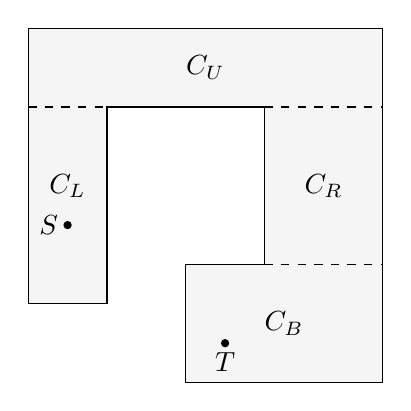
\begin{tikzpicture}[scale=.5]
\filldraw[fill=gray!8] (2,2)--(2,7)--(6,7)--(6,3)--(4,3)--(4,0)--(9,0)--(9,9)--(0,9)--(0,2)--cycle;
\draw[dashed] (0,7)--(2,7) (6,7)--(9,7) (6,3)--(9,3);
\node at (1,5){$C_L$};\node at (4.5,8){$C_U$};
\node at (7.5,5){$C_R$};\node at (6.5,1.5){$C_B$};
\fill (1,4) circle(3pt) node[left]{$S$};\fill (5,1) circle(3pt) node[below]{$T$};
\end{tikzpicture}
\caption{The spiral normal form, illustrated with separated arms. Dashed segments are open portals, never mirrors. The terminal source and target shown are the pair placement requiring the new four-band construction.}
\end{figure}

Define
\begin{align*}
 R_v&=A-w,& L_v&=R_v/(2c),\\
 N_{s,v}&=\lceil L_vh/(2a)\rceil+1,&
 N_{r,v}&=\lceil L_vh/(2R_v)\rceil+1,\\
 \delta_v&=L_v/(N_{s,v}+N_{r,v}+1).
\end{align*}
The transposed quantities are
\begin{align*}
 R_h&=H-h,& L_h&=R_h/(2a),\\
 N_{s,h}&=\lceil L_hw/(2c)\rceil+1,&
 N_{r,h}&=\lceil L_hw/(2R_h)\rceil+1,\\
 \delta_h&=L_h/(N_{s,h}+N_{r,h}+1).
\end{align*}

\begin{theorem}[Tall or wide spiral]\label{thm:tall}
Every distinct real interior pair in $P$ illuminates if either
\[
 H\ge c+2A/\delta_v\qquad\text{or}\qquad A\ge a+2H/\delta_h.
\]
There is no rationality or uniform reflection-count assumption.
\end{theorem}

\begin{theorem}[Coprime thin-cap lattice family]\label{thm:coprime}
Let $a$ be a positive integer, $N\ge5$ an odd integer, and $0<b<c<h$ integers with $c$ odd. Put
\[
 \ell=(N-2)a,\quad w=(N-1)a,\quad A=Na,\quad H=h+1.
\]
Every distinct actual interior pair in $(2\Z)^2$ illuminates in the room \eqref{eq:vertices}.
\end{theorem}

The second theorem concerns native even-even marks. It is not an all-real-endpoint theorem. The first theorem is all-real but has a sufficient metric restriction. Their hypotheses must not be merged.

\section{Protected endpoint placements}
We use the orientation-controlled L and U constructions in \cite{eightwall}. In an L room, paths can be chosen with only vertical, or only horizontal, reflections. The opposite-arm U construction has one floor reflection, otherwise vertical reflections, and monotonically decreasing arm heights toward the base. Its strict portal and corner guards include arm/base-level endpoints. These specific constructions, rather than a general enlargement principle, are the dependencies used below.

Set $Q=C_L\cup C_U\cup C_R$, a U room after $(x,y)\mapsto(x,H-y)$, and
\[
 R=([\ell,A]\times[0,c])\cup([w,A]\times[c,H]).
\]
Define
\[
 G=\intr P\cap\bigl(\{x<a,y>b\}\cup\{y\ge h\}\cup\{x>w,y\ge c\}\bigr).
\]
Every point in $G$ is interior to $Q$. The only artificial open wall of $Q$ is $x=w,0<y<c$. The U construction's used right-arm contacts are strictly above the right endpoint's original height, which is at least $c$; hence it avoids this wall and the extra physical corner $(w,c)$. Left-arm contacts have $y>b$, and cap contacts lie above $h$. Arm/base-level endpoints at $y=h$ use the actual U path, not a boundary segment across the notch. Arm-to-base placements use the vertical-only L construction. All used mirrors are genuine $P$ walls.

For two points strictly interior to $R$, use the horizontal-only L construction. Its horizontal mirrors $y=0,c,H$ are genuine $P$ walls. The artificial vertical cut $x=w$ above $h$ and its extra physical corner $(w,h)$ are never contacted. The disjunction in \eqref{eq:geometry} ensures that the left arm does not cover the bottom ledge.

Every actual point outside $G$ lies in $\{\ell<x<A,0<y<c\}\subset\intr R$. A point outside $\intr R$ lies in the actual left column or in the upper cap with $x\le w$. Therefore the only pairs not covered by these two protected constructions, up to reversal, are
\begin{gather}\label{eq:residual}
 T=(t,v),\quad\ell<t<A,\quad0<v<c,\\
 S=(s,u)\text{ with }0<s<a,\ b<u<h,
 \quad\text{or }h\le u<H,\ 0<s\le w,
 \quad S\in\intr P.\nonumber
\end{gather}
At $u=h$, actual interiority requires $s<a$. The upper cut $s=w,u>h$ remains an interior endpoint, not a mirror.

\section{A strict slope window for every residual target}
Write $R_v=R_0$, $L_v=L_0$ temporarily, and put
\[
 B=A-\ell>R_0,\qquad z=A-t\in(0,B),\qquad d=c-v\in(0,c),\qquad e=h-v\in(0,h).
\]
The reverse bottom phase $z_2(\tau)=z-d\tau$ lies in the strict right portal when $|z_2|<R_0$. Its positive-slope interval is
\[
 W=\left(\max\{0,(z-R_0)/d\},(z+R_0)/d\right).
\]
Its length exceeds $R_0/c=2L_0$. If $q=\max\{0,(z-R_0)/d\}$, then
\[
 J=(q+L_0/2,q+3L_0/2)
\]
has length $L_0$, positive slopes, and closure inside $W$.

For a lower-column source, remove source boundaries $s+(h-u)\tau=(2n+1)a$. They are spaced by $2a/(h-u)>2a/h$, so at most $N_{s,v}$ occur in $J$. Remove right-arm boundaries $z-e\tau=(2j+1)R_0$; at most $N_{r,v}$ occur there. For an upper-cap source only the latter boundaries are needed. One remaining open component $I=(\alpha,\beta)$ has length at least $\delta_v$. On it the integers $n,k$ are fixed and
\[
 z_0=s+(h-u)\tau-2na\in(-a,a),\qquad
 z_1=z-e\tau+2kR_0\in(-R_0,R_0),
\]
with $z_0$ used only for lower-column sources.

Let $D=2H-u-v$. Under the tall condition, $D>H-c\ge2A/\delta_v$. Define $C=2na+A+2kR_0+z-s$ in the lower-column case and $C=A+2kR_0+z-s$ in the upper-cap case. The target roots
\[
 \tau_m=(C+2mA)/D,\qquad m\in\Z,
\]
have spacing $2A/D<\delta_v$. Explicitly,
\[
 m=\left\lfloor\frac{D\alpha-C}{2A}\right\rfloor+1
\]
gives $\alpha<\tau_m\le\alpha+2A/D<\beta$. Thus the same slope satisfies all strict portals and the exact target equation, with the already fixed source/right indices.

\section{The four-band curve and roof-corner exclusion}
Let $F_q(x)=\dist(x,2q\Z)$ and use increasing developed height $\eta$; actual height rises to $H$ and then decreases. Set $\eta_1=2H-h$, $\eta_2=2H-c$.
For a lower-column source use
\begin{equation}\label{eq:fourbands}
 x(\eta)=\begin{cases}
 F_a(s+\tau(\eta-u)),&u\le\eta\le h,\\
 F_A(z_0+\tau(\eta-h)),&h\le\eta\le\eta_1,\\
 A-F_{R_0}(z_1+\tau(\eta-\eta_1)),&\eta_1\le\eta\le\eta_2,\\
 A-F_B(z_2+\tau(\eta-\eta_2)),&\eta_2\le\eta\le2H-v.
 \end{cases}
\end{equation}
The target equation gives
\[
 z_0+2(H-h)\tau-(2m+1)A=z_1,\qquad
 z_1+(h-c)\tau-2kR_0=z_2.
\]
The final bottom argument is exactly $z$, hence the final point is actual $T$.
At each portal the strict residual bound makes the adjacent folds agree locally, including signed velocity: subtract even source/right periods or an odd cap multiple of $A$. A zero residual represents one smooth outer-wall reflection, not an artificial turn.

All open-band mirrors are genuine: $x=0,a$ in the left column, $x=0,A$ above $h$, $x=w,A$ in the right arm, and $x=\ell,A$ below $c$. Strict residuals exclude every ledge corner. If the roof contact were a convex corner, the cap phase there would be an integer multiple of $A$. Symmetry about that cusp would make the two cap-portal abscissae equal. The first is in $[0,a)$, the second in $(w,A]$, impossible. There are finitely many contacts since all slopes, times and widths are finite.

For an upper-cap source, replace the first two bands by $F_A(s+\tau(\eta-u))$ from $u$ to $\eta_1$; the last two remain as in \eqref{eq:fourbands}. If its roof contact is smooth, the proof is complete. If it is a corner, write $q=s+\tau(H-u)\in A\Z$. At $\eta=2H-u$ the cap phase is $2q-s$, so the folded curve returns to the \emph{same actual} $S$. For $u>h$ this precedes the right portal and the target. Discard the entire earlier part, including the singular contact, and launch along the legal descending suffix from that interior occurrence of $S$. Its remaining contacts are already guarded and it never returns to the roof. For $u=h$ such a return would have $x=s\le w$ at the second portal, contradicting its strict $x>w$ guard, so the singular case cannot occur.

For lower-column sources, no earlier target is met on the ascending part: if $\ell\ge a$, then $x<a<t$; if $\ell<a$, separation forces $c<b$ and the source portion has $y\ge u>b>c>v$. Cap heights exceed $v$, and descending height reaches $v$ only at its end. The actual endpoint is therefore retained. This proves the tall half of Theorem~\ref{thm:tall}.

Swapping coordinates and reversing the boundary traversal gives the same normal form with
\[
 (a',\ell',w',A',b',c',h',H')=(c,b,h,H,\ell,a,w,A).
\]
The separation condition becomes $c<b$ or $a<\ell$, unchanged. Apply the tall theorem in this isometric room and swap the actual endpoints back. Its threshold is exactly the wide condition, completing the proof.

\section{Coprime periods: the terminal lemma}
Now take rational $a>0$, equal terminal arm widths $a$, bottom width $2a$ and cap width $A=Na$, with $N\ge5$ odd and integers $0<b<c<h<H$. Let $S=(s,u)$ be a rational terminal source with $0<s<a$, $b<u\le h$, and $T=(t,v)$ a rational bottom target with $\ell<t<A$, $0<v<c$. Assume $u,v$ are integers and $d_2=c-v$ is odd. Put
\[
 d_0=h-u\ge0,\quad G=2(H-h)>0,\quad g_1=h-c>0,\quad
 D=d_0+G+g_1+d_2=2H-u-v,
\]
and assume $\gcd(G,N)=1$. Write $z=A-t\in(0,2a)$.

\begin{lemma}\label{lem:terminal}
Under these assumptions, $S$ illuminates actual $T$.
\end{lemma}
\begin{proof}
Start from the target-compatible slope grid
\[
 \tau_q=(A+z-s+2aq)/D,\qquad q\in\Z.
\]
Let $t_1=d_0$, $t_2=d_0+G$, $t_3=D-d_2$. Avoid the three congruences
\begin{align*}
 s+t_1\tau_q&\equiv a\pmod{2a},\\
 s+t_2\tau_q-A&\equiv a\pmod{2a},\\
 s+t_3\tau_q-A&\equiv a\pmod{2a}.
\end{align*}
If $t_1=0$, its congruence is impossible since $0<s<a$. Each nonzero-time congruence is either empty or a single residue class of integers $q$ modulo $m_i=D/\gcd(t_i,D)\ge2$. Nonzero times are distinct and strictly between $0$ and $D$, so at most one has modulus two.

Three single residue classes with moduli at least two can cover $\Z$ only if two moduli are two, or all three are three, or the multiset is $(2,4,4)$. For completeness: minimum at least four gives total density at most $3/4$; minimum three requires all three to be three by density. With minimum two and second at least five, density is less than one. With second four, the third must four. With second three and third at least four, the first two cover $2/3$ and the third cannot fill the complement; third three gives at most $5/6$.

Two moduli two would require two equal times $D/2$. Three moduli three would require three distinct times chosen from $D/3,2D/3$. Both are impossible. For $(2,4,4)$, increasing time order forces $(t_1,t_2,t_3)=(D/4,D/2,3D/4)$, so $G=d_2=D/4$, contradicting even $G$ and odd $d_2$. With $t_1=0$, at most two classes remain and their distinct nonzero times cannot both have modulus two. Thus the forbidden classes do not cover $\Z$. All their moduli divide $D$, so choose $q\in\{0,\ldots,D-1\}$ avoiding all events. Its slope $\tau_0>0$.

Let $n=\lfloor(s+d_0\tau_0+a)/(2a)\rfloor$ and $z_0=s+d_0\tau_0-2na$. The first exclusion gives $|z_0|<a$. Replacing $\tau_0$ by $\tau=\tau_0+2aM$ leaves $z_0$ unchanged, since $d_0$ is integral. As $M=0,\ldots,N-1$, the cap phase $X=z_0+G\tau$ modulo $2A$ visits all $N$ points of a coset with spacing $2a$, because $\gcd(G,N)=1$.

The open return window $X\in(2m+1)A+(-a,a)$ modulo $2A$ has length $2a$. Its endpoints are avoided by the second congruence exclusion. Exactly one of the coset points lies strictly inside it. Select that $M,m$ and put $z_1=X-(2m+1)A$, so $|z_1|<a$. Define
\[
 k=\left\lfloor\frac{z_1+g_1\tau+a}{2a}\right\rfloor,\qquad
 z_2=z_1+g_1\tau-2ka.
\]
The third exclusion, unchanged by the integral slope shift, gives $|z_2|<a$.

The final bottom phase is
\[
 E=z_2+d_2\tau=s+D\tau-2na-(2m+1)A-2ka=z+2aJ
\]
for an integer $J$. If $J$ is odd, increase $\tau$ once more by $2aN$. Then $n$ increases by $Nd_0$, $m$ by $G$, and $k$ by $Ng_1$. All three strict residuals stay unchanged, while $E$ increases by $2aNd_2$. Since $N,d_2$ are odd, this flips $J$'s parity. After at most one correction $E\equiv z\pmod{4a}$, so $F_{2a}(E)=z$ exactly.

Use the four-band formula \eqref{eq:fourbands}, now with $R_0=a$ and $B=2a$, from $\eta=u$ to $2H-v$. The first band is empty for $u=h$, with $z_0=s$. Strict residuals match the actual portals and signed velocities. All open-band mirrors are genuine. A roof-corner event would equate cap portal abscissae in $[0,a)$ and $(w,A]$, impossible. The terminal phase is exactly the actual $t=A-z$. The ascending portion has $x<a<\ell<t$, so it cannot meet the target earlier. All choices and contacts are finite. This proves the lemma.
\end{proof}

\section{The whole thin-cap native-pair family}
Under Theorem~\ref{thm:coprime}'s assumptions, $G=2$ is coprime to odd $N$. An even-even left-terminal mark has integer height $u<H=h+1$, hence $u\le h$. A bottom mark has even height $v$, so $c-v$ is odd. Every residual terminal pair therefore satisfies Lemma~\ref{lem:terminal}, including $u=h$.

There is no integer-height mark strictly inside the cap band $h<y<h+1$. Thus the protected coverage of Section 2 leaves only a left-terminal versus bottom-terminal native pair. The lemma covers that pair, and path reversal covers the opposite labeling. This proves Theorem~\ref{thm:coprime}.

For example, $(a,\ell,w,A;b,c,h,H)=(4,12,16,20;1,5,7,8)$ meets the arithmetic hypotheses, but the tall and wide thresholds require respectively $H\ge505$ and $A\ge644$. The arithmetic theorem therefore adds coverage outside both sufficient metric conditions. This example illustrates a proved infinite-family statement; finite path checks alone would not prove it.

\section{Dependencies and remaining scope}
The protected L/U constructions are imported from \cite{eightwall} with the precise orientation and wall-avoidance properties used in Section 2. All other existence steps are the finite interval and congruence arguments given here. Source arguments are \texttt{three-reflex-argument-01.md}, \texttt{three-reflex-argument-03.md}, \texttt{three-reflex-argument-04.md} and \texttt{coprime-proof.md}; their exact versions and scoped reviews are listed in the accompanying README and \texttt{provenance.json}.

Other arithmetic supplements have additional hypotheses and are not silently included. The complementary arbitrary-real metrics, other ten-wall normal forms and a universal 22-wall minimum remain open. No darkness follows from failure of a sufficient condition. This draft has not been externally refereed or checked in a proof assistant.

\begin{thebibliography}{9}
\bibitem{eightwall} D. Wang and P. Wang, \emph{Illumination of orthogonal rooms with at most eight walls}, working draft v0.1 (2026), Sections 2--3. Included as \path{preprints/eight-wall/manuscript.pdf} in \url{https://github.com/peytonprogrammer/illumination-problem}.
\end{thebibliography}

\smallskip\noindent\textbf{Acknowledgments.} The authors used AI tools, including OpenAI Codex and Anthropic Claude, to develop and revise this research, its theorem proofs, and the manuscript. The authors remain responsible for the content.
\end{document}
